% Template for ICASSP-2013 paper; to be used with:
%          spconf.sty  - ICASSP/ICIP LaTeX style file, and
%          IEEEbib.bst - IEEE bibliography style file.
% --------------------------------------------------------------------------
\documentclass{article}
\usepackage{spconf,amsmath,graphicx,bm,setspace}
\usepackage{todonotes}
\setlength{\marginparwidth}{1.5cm}
\usepackage{lipsum}
\usepackage{multirow}
\usepackage{threeparttable}
\usepackage{caption}
\usepackage{subcaption}

\sloppy
\renewcommand{\normalsize}{\fontsize{8.7}{10.7}\selectfont}

% ADD THE FOLLOWING COUPLE LINES INTO YOUR PREAMBLE
\let\OLDthebibliography\thebibliography
\renewcommand\thebibliography[1]{
  \OLDthebibliography{#1}
  \setlength{\parskip}{0pt}
  \setlength{\itemsep}{0pt plus 0.3ex}
}

% Example definitions.
% --------------------
\def\x{{\mathbf x}}
\def\L{{\cal L}}

% Title.
% ------
\title{Transfer learning between concepts for human behavior modeling: An application to sincerity and deception prediction}
%
% Single address.
% ---------------
\name{Qinyi Luo$^+$, Rahul Gupta$^o$, Shrikanth Narayanan$^o$}
\address{ $^+$Department of Electronic Engineering, Tsinghua University, Beijing, China \\
$^o$Signal Analysis and Interpretation Lab, University of Southern California,  Los Angeles, CA, USA}  
\begin{document}
\ninept
%
\maketitle
%
\begin{spacing}{0.89}
\begin{abstract}
Transfer learning (TL) involves leveraging information from an external source for enhancing model performances for a problem at hand. 
Popular TL methods either directly use the data or adapt the models learned on out-of-domain resources and incorporate them within in-domain models. 
TL methods have shown promise in several applications such as text classification, cross-domain language classification and emotion recognition.
In this paper, we propose TL methods to computational human behavioral trait modeling. Many human behavioral traits are abstract constructs (e.g., sincerity of an individual), and are often conceptually related to other constructs (e.g., level of deception) making TL methods an attractive option for their modeling. We consider the problem of automatically predicting human sincerity and deception from behavioral data while leveraging transferal of knowledge from each other. 
%We investigate several TL methods including appending datapoints from the other dataset as well as appending sincerity/deception predictions as features from models learnt on the other dataset. 
%These approaches are based on the hypotheses that sincerity perception and deceptive intent labels carry certain correlation between them and one could be leveraged during model training for the other. 
We compare our methods against baseline models trained only on in-domain data.
Our best models achieve an Unweighted Average Recall (UAR) of 72.02\% in classifying deception (baseline: 69.64\%). 
Similarly, applied methods achieve Spearman's/Pearson's correlation values of 49.37\%/48.52\% between true and predicted sincerity scores (baseline: 46.51\%/41.58\%), indicating the success and the potential of TL for such human behavior tasks.
 
\end{abstract}
%
\begin{keywords}
Transfer Learning (TL), sincerity prediction, deception prediction 
\end{keywords}
%
\vspace{-3mm}
\section{Introduction}
\vspace{-3mm}
\label{sec:intro}
Transfer Learning (TL) focuses on learning knowledge from one domain and applying it to other related domain \cite{pan2010survey}. 
TL has shown promise in several research fields such as mining text data \cite{aggarwal2012mining}, reinforcement learning \cite{taylor2009transfer} and natural language understanding \cite{blitzer2007biographies}.  
In particular, domains with limited resources (e.g. absence of a comprehensive datasets) can gain from TL approaches as it is possible to learn models on a related problem and adapt the models to domain of interest. 
Human behavior modeling \cite{luo2008agent,narayanan2013behavioral} is one such domain where obtaining reliable (human) annotations on large datasets is both expensive and prohibitive in time.
In this paper, we consider the problems of modeling deceptive intent (deceptive vs not-deceptive) and rating perceived sincerity; applying TL methods in assisting one problem using resources from the other. 
We hypothesize that the perception of sincerity and deceptive intent carry certain conceptual relation in their behavioral manifestations, and therefore resources in one domain can enhance performance in the other domain.
We test multiple TL methods such as using data from the other domain, using model predictions from the other domain as well as the combination of the two aforementioned TL approaches. 
Our experiments target the overarching goal of enhanced human behavior modeling by sharing resources across various related problems and possibly learning a joint representation for various behavioral attributes. 

%Studies have investigated and proposed several TL approaches \cite{pan2010survey} and one of the earliest works in TL was proposed by Pratt \cite{pratt1993discriminability}.
Several transfer learning approaches have been proposed \cite{pan2010survey}, with one of the earliest appearing by Pratt \cite{pratt1993discriminability}. 
More recent TL approaches include TL via dimensionality reduction \cite{pan2008transfer}, using deep learning representations \cite{bengio2012deep, mesnil2012unsupervised} and transfer learning in a transductive setting \cite{rohrbach2013transfer}.  
TL methods have been applied to sentiment classification \cite{blitzer2007biographies}, image classification \cite{wu2004improving} and other natural language understanding problems \cite{arnold2007comparative,blitzer2006domain}. 
Recently, TL methods have been applied to modeling human behavior such as emotion recognition \cite{zhang2016enhanced}, facial expression recognition \cite{chen2013learning} as well as analysis \cite{sangineto2014we}.

Within the domain of sincerity and deception prediction, several modeling schemes were presented as part of the Interspeech 2016 Computational Paralinguistics Challenge \cite{schuller2016interspeech} including DNN rank learning \cite{gabor2016sinc}, learning using phone recognition based features \cite{herms2016sinc} and fusion of acoustic feature representations \cite{kaya2016sinc}.  
As a part of the challenge, Zhang et al. \cite{zhang2016sinc} proposed a transfer learning approach with multi-task learning perspective.
%{\bf Add a sentence about zhang et al. and say how our algo is different after seeing that paper at IS.} 
Their proposal involves label generation for the task at hand from out-of-domain unlabeled data and retraining the model, a methodology also explored in our experiments.
However, we explore additional domain adaptation to account for differences in the two datasets. 
Moreover, Zhang et al. \cite{zhang2016sinc} modify the continuous sincerity scores into binary labels for label compatibility.
In our work, we retain the original sincerity and deception labels, thereby exploring methods that extend to labels with different granularity. 

The TL methods tested in our experiments are based on the hypotheses that sincerity and deception are related, with deceptive sentences being more likely to be perceived as insincere and vice versa. 
Research in psychology has investigated the two concepts of sincerity and deception in various contexts such as integrity \cite{mcfall1987integrity}, leadership \cite{stinchfield1936sincerity} and interpersonal perceptions \cite{toris1984effects}. 
Often these concepts are seen to oppose each other with low sincerity implying a deceptive intent. 
We test our models based on this hypothesis on the Deceptive Speech Database and Sincerity Speech Corpus made available during the Interspeech challenge 2016 \cite{schuller2016interspeech}.
Initially, we train baseline models from in-domain resources without using any TL from the other dataset. 
This is followed by testing various settings of TL categorized as: (i) using datapoints from the other dataset and, (ii) appending sincerity/deception predictions from the other model as features.
Finally, we also combine the two approaches and test using datapoints from the other dataset as well as sincerity/deception predictions from other model as features.
The best models achieve an Unweighted Average Recall of 72.02\% (baseline: 69.64\%) on classifying deceptive vs non-deceptive intent and Spearman's/Pearson's correlation coefficients of 49.37\%/48.52\% (baseline: 46.51\%/41.58\%) between true and predicted sincerity scores.
Finally, we analyze the results and present our conclusions. 
In the next section, we introduce the datasets followed by the description of our methodology in Section 3.

%This paper is organized as follows: Section 2 presents the dataset, followed by the description of baseline and various TL methodologies in Section 3.
%We present the results in Section 4 and the final conclusions and future steps are presented in Section 5.

\vspace{-3mm}
\section{Datasets}
\vspace{-3mm}
%Two databases from the INTERSPEECH 2016 Computational Paralinguistics Challenge are employed in the experiments, the Deceptive Speech Database (DSD) and the Sincerity Speech Corpus (SSC). For both databases, samples outside of the test set are accessible, constituting the datasets for our experiments, denoted as the D dataset and the S dataset respectively. For both datasets, the official ComParE Acoustic Feature Set was used, containing 6373 static features computed over low-level descriptor contours. For more information about the Challenge, please refer to [x].\par
%Descriptions of the two datasets are detailed below.

%\subsection{D dataset}
%The DSD was produced at the University of Arizona, consisting of 1556 speech samples from 72 speakers recorded in structured interviews. A total of 1059 samples are contained in the D dataset. For each sample, the label is either Deceptive (D) or Non-Deception (ND). In the Deceptive condition, participants were asked to lie about their identity and behavior, while in the Non-Deceptive condition, they were asked to tell the truth. The interviews were carried out by an Embodied Conversational Agent (ECA) in order to ensure consistency.

%\subsection{S dataset}
%The SSC provided by the Columbia University contain 655 available speech instances from 22 speakers and 256 instances held confidential by the Challenge. All of the 655 available instances were included in the S dataset. When recording the instances, a number of participants were asked to read six different sentences, each sentence in 4 different styles (monotonic, non-monotonic, fast and slow). Each instance was graded from 0 to 4 by at least 13 human annotators regarding perceived sincerity, with higher scores indicating more sincerity. Scores given by the same annotator were normalized to zero mean and unit standard deviation. Averaging the normalized scores from all annotators, a sincerity rating was obtained for each instance.

%\subsection{Comparisons between datasets D and S}
%The D dataset and the S dataset are linked together by the complementary relationship between deception and sincerity. Certain similarities are expected to exist between Deceptive samples and instances in the S dataset with low sincerity scores, and also between Non-deceptive samples and highly sincere instances.\par
%Nevertheless, in terms of recording conditions, the two datasets are hardly alike. 
%Speech samples in the D dataset are more similar to natural speech, as the subjects were allowed to arrange speech and show emotions freely. On the contrary, participants for the S dataset were subjected to more restrictions, resulting in more acting. Moreover, labels for the D dataset are objective and binary, while sincerity ratings are subjective and continuous.\par
%The aforementioned differences pose challenge to transferring knowledge from one dataset to the other. On the other hand, they help simulate a real-world inter-concept knowledge transfer situation, where little consistency is guaranteed between corpora.

We use two datasets for the purpose of our experiments: (i) Deceptive Speech Dataset and, (ii) Sincerity Speech Corpus.
Both these datasets were made available as part of the Interspeech 2016 computational paralinguistic challenge \cite{schuller2016interspeech}.
We would like to state that we make use of datasets partitions labeled as training and development set during the challenge, as the testing set labels were not released.
Our models are evaluated using a cross-validation framework on the data portion with the availability of labels. 
We briefly describe the two datasets below.\\ 

\noindent{\bf Deceptive Speech Dataset (DSD)}:
The DSD dataset is available from the University of Arizona and we use a set of 1059 speech samples obtained from 49 participants.
In each of these samples, the participant either lies about his identity and behavior or tells the truth. 
Therefore, each of these samples is associated with a binary label of the speech being deceptive or not.
747 utterances (out of 1059) are marked as non-deceptive in the dataset.
We refer the reader to \cite{schuller2016interspeech} for further details on this dataset.\\

\noindent{\bf Sincerity Speech Corpus (SSC)}:
We use the SSC dataset provided by the Columbia University, consisting of 655 speech samples from 22 speakers.
Unlike the labelling schemes for the DSD dataset, the samples in the SSC dataset are rated for perceived sincerity by a group of 13 annotators in a range of 0-4. 
The scores for each annotator were further normalized to zero mean and unit standard deviation.
The final sincerity score for each sample is computed as the mean of thus normalized sincerity score from each annotator.
Further details regarding the dataset are available in \cite{schuller2016interspeech}.

The goal of our experiments is to utilize the expected relationship between deception and perceived sincerity labels.
We hypothesize the deceptive utterances would have a low perceived sincerity, and also, utterances with low perceived sincerity are more likely to be deceptive.
Therefore, in order to improve the performance for one dataset, we aim to utilize the knowledge from the other dataset by either directly using the datasamples from that dataset or using the model learnt on the other dataset.
However, ensuring the maximal transfer of knowledge from one dataset to the others is not trivial due to several dissimilarities between the datasets.
These dissimilarities exist in the form of differences in dataset collection conditions and protocols, annotation procedures and the nature of labels.
To begin with, we do not have any indication of (continuous) sincerity labels on DSD dataset and (binary) deception labels on the SSC dataset.
Also, the speech samples in the DSD dataset are more similar to natural speech, as the subjects were allowed to arrange speech and show emotions freely. 
On the contrary, participants for the SSC dataset were asked to utter pre-specified sentences. 
%Moreover, labels for the DSD dataset are objective and binary, while sincerity ratings in the SSC dataset are subjective and continuous.
We address these issues using a few label generation and data transformation techniques.
The label generation and data transformation are performed using features extracted on each of the two datasets.
We describe these features in the next section.

\vspace{-3mm}
\subsection{Features}
\vspace{-2mm}
\label{sec:feats} 
We extract a common set of 6373 acoustic features on the DSD and SSC datasets, termed as the ComParE Acoustic Feature Set \cite{weninger2013acoustics}. 
These features were also used in the Interspeech challenge baseline \cite{schuller2015interspeech,schuller2016interspeech}.
These features are statistics computed on energy related descriptors (e.g. loudness, RMS energy, zero crossing rate), spectral descriptors (e.g. Mel Frequency Cepstral Coefficients, spectral energy) and voicing related descriptors (e.g. F0, voicing probability).
Further details on these features can be obtained from \cite{weninger2013acoustics}. 

\vspace{-3mm}
\section{Methodology}
\vspace{-3mm}
%In the experiments, we first determined the baselines by training and testing on the two datasets separately. Then we transferred knowledge between the two datasets, during which process data information as well as label information of one dataset can be utilized to enhance affect computing on the other dataset. We experimented with 3 knowledge transfer methods. The first method was the Random Sample Consensus (RANSAC) algorithm, which utilized data information in the transfer, but ignored label information. The second method tried to utilize both data and label information via label transformation. Compared to these 2 methods, we proposed a novel method that exploited both data and label information and produced better results.\par
%For classification on the D dataset, unweighted average recall (UAR) was measured. For regression on the sincerity ratings, Spearman's correlation was computed.
%For ease of exposition, in the rest of this paper, premodifier 'D' indicates relation to the D dataset or deception identification, while premodifier 'S' implies relation to the S dataset or sincerity evaluation.

The goal of experiments is to exploit the information from one dataset for improved target prediction on the other dataset.
For the purpose of this demonstration, we initially set a baseline on each of the two datasets.
We then conduct two categories of experiments to utilize the information from a given dataset in improving performance for the other dataset. 
In the first set of experiments, while predicting the target labels for the dataset at hand, we add the datapoints from the other dataset with labels of interest generated synthetically. 
In the second experiment, we use the outputs from a sincerity prediction model as features during deception prediction and vice versa.
Finally, we combine the two schemes of adding data and using predictions from the other model.
Below, we describe each of these modeling schemes in detail. 

\vspace{-2mm}
\subsection{Baseline experiments}
\vspace{-2mm}
%For deception detection, a classifier was trained on the D dataset using SVM classification. Ten-fold cross validation was implemented, with 1 fold as the test set, 1 fold as the development set and the rest as the train set. Z-scores were taken on all features with the mean and standard deviation computed on the corresponding train set. We tuned the box constraint on the development set, and tested the results using a model trained on the concatenated train and development sets with the optimal box constraint.\par
%For sincerity evaluation, a regressor was trained on the S dataset using SVM regression. A leave-one-speaker-out cross-validation schema was adopted. In each fold, the test set contained one speaker's speech samples, while the train set had 9 speakers and the development set had 12. All labels were scaled to range from -1 to 1. Z-scores were taken on all features with the mean and standard deviation computed on the corresponding train set. The cost parameter was tuned on the development set. To obtain the test set performance, we trained a model on the concatenated train and development sets using the optimal cost parameter.

In the baseline systems, we only use the datapoints corresponding to each individual dataset, without any transfer of knowledge between the SSC and DSD datasets.
We describe the choice of baseline modeling schemes for the deception and sincerity prediction below.
%\\

%\noindent
\underline{\it Deception prediction}: 
We train a Support Vector Machine (SVM) classifier on the ComParE Acoustic Feature Set \cite{weninger2013acoustics} to predict the binary label of an utterance being deceptive or not.
Same classifier was also used in the baseline presented in the Interspeech challenge 2016 \cite{schuller2016interspeech}.
For evaluation purpose, we perform a 10 fold cross-validation, each fold containing an independent set of speakers.  
8 partitions are used as training set, 1 as development set and 1 as testing set.
SVM parameters such as kernel and box-constraint are tuned on the development set.
We use Unweighted Average Recall (UAR) as the evaluation metric on the DSD dataset, as was also the case during the Interspeech challenge 2016 \cite{schuller2016interspeech}.
UAR assigns equal weight to each class during recall computation, a case helpful when the class distribution is biased. 
The baseline results are listed in Table~\ref{tab:results}.
Note that the results are slightly different than the one presented in the Interspeech 2016 challenge paper \cite{schuller2016interspeech} as their evaluation defined a different partitioning scheme for the development and the testing set.
%\\

%\noindent
\underline{\it Sincerity prediction}:
Since the sincerity prediction involves continuous labels, we train a Support Vector Regressor (SVR) as the predictor (same regressor model was used during the Interspeech challenge 2016 \cite{schuller2016interspeech}).
We use evaluation metrics as both Spearman's and Pearsons's correlation to obtain a sense of relative ordering as well as linear correspondence between predicted and true labels. 
In the baseline experiment, we perform a finer leave one speaker out cross-validation due to a small number of datasamples.
Apart from the speaker in the testing set, other speakers are roughly equally divided between the training and the development set.
The parameters for the SVR (kernel and box-constraint) are tuned on the development set. 
Table~\ref{tab:results} presents the baseline results.
The results are slightly different from the ones presented in the Interspeech 2016 challenge paper \cite{schuller2016interspeech} due to differences in data partitioning and the fact that in the Interspeech challenge, the box-constraint parameter was tuned globally for each fold.
We, on the other hand, find the best parameters for each fold independently based on the development set. 

\vspace{-2mm}
\subsection{Transfer Learning (TL)}
\vspace{-2mm}
Using TL, we aim to leverage one dataset for an improved performance on the other dataset.
We propose two TL experiments, namely: (i) adding datapoints from the other dataset during training and, (ii) appending sincerity/deception predictions from the other model as features.
In the first approach, we expect that adding datapoints from the other dataset with synthetically created labels provides a lower generalization error \cite{vapnik1998statistical}.
In the second approach, we use sincerity predictions to improve classification of deception prediction (likewise using deception prediction for sincerity scoring). 
These approaches aim to exploit the hypotheses that there exists a relation between the sincerity and deception labels, therefore one can be used a predictor for the other.
We describe the experiments in detail below. 

\vspace{-2mm}
\subsubsection{TL: adding datapoints from the other dataset during training}
\vspace{-2mm}
%Based on the baselines, the knowledge transfer experiments aimed to improve the performance on one dataset with the help of the other dataset. To allow fair comparison, some procedures remained unchanged: (a) when training D classifiers, ten-fold cross validation was implemented in the same way as in the baselines, and the box constraint was tuned on the development set; (b) when obtaining S regressors, leave-one-speaker-out cross validation was adopted as in the baselines, and the best cost parameter was chosen on the development set.

In this section, we append the datapoints from the other dataset in order to improve the performance for the task of interest.
First, we generate synthetic labels for the task at hand for each datapoint in the other dataset.
These datapoints and synthetic labels are then added to the datapoints and the labels of the original dataset for final model training.
We test two synthetic label generation algorithms: Random Sample Consensus (RANSAC) and label transformation.
We discuss these algorithms in detail below.
\\

\noindent{\bf(a) Random Sample Consensus (RANSAC)}:
%One way to transfer knowledge is to add one dataset as unlabeled data to the other dataset in hope that more data points will generate better results. In light of this, we implemented the RANSAC algorithm.\par
%RANSAC is an iterative algorithm. Starting from a small set of data points (the initial dataset), it enlarges the dataset by adding consistent data points and renews the model in each iteration. In an extreme case of RANSAC, the unlabeled data can be added into the initial dataset all in one iteration. More information about RANSAC can be found in [x].\par
%In our experiments, one of the D and S datasets served as the initial dataset, and the other dataset was treated as unlabeled data to be added. Z-scores were taken on both datasets to reconcile possible differences in data characteristics that resulted from recording conditions.\par
%For classification on the D dataset, the D train set served as the initial dataset, on which the initial classifier was instantiated. The S dataset was the initial unlabeled dataset. In each iteration, the classifier predicted labels for the unlabeled dataset. Data points that were far away from the decision hyperplane were added into the initial dataset and removed from the unlabeled dataset. A renewed classifier was then trained on the enlarged dataset. When adding the data points in each iteration, three different criteria were applied: (a) data points that were the farthest 5 percent away from the decision hyperplane were added; (b) data points that were the farthest 10 percent away from the decision hyperplane were added; (c) all of the unlabeled data points were added. To stop the iteration, either one of the following two conditions were required: (a) the performance on the development set was stable; (b) the unlabeled dataset was empty. To test the results, we selected the classifier from the iteration in which the performance on the development set was the highest.\par
%For regression on the S dataset, the D dataset was gradually added into the S dataset. An initial regressor was trained on the S train set. In each iteration, the unlabeled D data points were grouped into several clusters using k-means clustering. The number of clusters was determined using the silhouette method. Then one cluster was selected to add into the initial dataset by the following procedure: (a) each cluster was added into the initial dataset respectively, and regressors were trained on the augmented initial datasets. Therefore each cluster resulted in one regressor; (b) The new regressors were used to predict labels for the corresponding initial dataset, and root mean square errors were computed; (c) The cluster with the smallest corresponding root mean square error was selected. The selected cluster was then added into the initial dataset and excluded from the unlabeled dataset. The stopping criteria were the same as for the classification on the D dataset: (a) the performance on the development set was stable, or (b) the unlabeled dataset was empty. We also tried the extreme case of RANSAC, where the D dataset was added into the S train set all in one iteration. Judging from the performance on the development set, the best regressor among all iterations was used to obtain results on the test set.
During the RANSAC \cite{fischler1981random} implementation, an initial model is trained on the available dataset with labels.
Then, the algorithm performs prediction on the datapoints from the other dataset without the labels of interest.
A fraction of these datapoints is then added to the existing labeled dataset and an updated model is trained with the additional labeled data.
Researchers have proposed several criteria for selecting the fraction of data (e.g. adding the datapoints farthest away from class boundaries).
This procedure is repeated iteratively till a certain criterion is met (in our experiments, we perform the iterations till the performance on the held out development set is maximized).
Studies have investigated the use of RANSAC in several applications including image analysis \cite{fischler1981random} and compute graphics \cite{caraiman2009new}. 
Since the task objective is different for the DSD and the SSC corpus, we describe them separately below. 
%\\

%\noindent
\underline{\it Deception prediction}:  
For the purpose of deception prediction, synthetic labels are obtained on the SSC dataset.
We use the same train, test and development set split as in the baseline experiments.
Initially, an SVM model is obtained using the train partition of the DSD dataset and datapoints are added from the SSC dataset till the performance on the development partition of the DSD dataset is maximized.
In each iteration, datapoints farthest away from the class boundary are added \cite{raguram2008comparative}.
We tune the proportion of SSC data added at each iteration from farthest 5\% to all of the data.
%\\

%\noindent
\underline{\it Sincerity prediction}: 
The details of sincerity prediction are similar to deception prediction, except for the fact that the model we train is an SVR.
We implement the regression version of RANSAC algorithm as proposed in \cite{raguram2013usac}, where a cluster of points with least prediction error using the existing regression model is added iteratively. 
The train, test and development set partitions are kept the same as the baseline experiments.
Table~\ref{tab:results} shows the results for the RANSAC algorithm implementation.
\\

\noindent{\bf (b) Label transformation}:
%In an attempt to incorporate label information when appending one dataset to the other, we transformed the labels to achieve compatibility between binary and continuous labels. Z-scores were taken on both datasets to reconcile possible differences in data characteristics that resulted from recording conditions.\par
%For classification on the D dataset, the continuous S labels were binarized, and the S dataset was appended to the D train set along with the new labels. Binarization was achieved by comparing sincerity ratings to a threshold $V_{th}$, i.e. samples whose sincerity ratings were lower than $V_{th}$ were labeled as Deceptive while others were labeled non-deceptive. A classifier was trained on the enlarged train set, and the threshold was tuned on the development set. Using the optimal threshold and the optimal box constraint, we obtained the test set performance using a classifier trained on the concatenated train and development sets, which included the original train and development sets as well as the S dataset.\par
%For regression on the S dataset, we assigned different values to D and ND labels, i.e. all deceptive samples were given a sincerity rating $v_{1}$ while the non-deceptive samples were graded $v_{2}$. We enlarged the S train set by adding the D dataset, and tuned $v_{1}$ and $v_{2}$ on the development set. Results on the test set were tested using a regressor trained on the concatenated train and development sets.
Previously, we hypothesized that there exists a relation between the sincerity and the deception labels.
The RANSAC algorithm does not make use of sincerity labels during training deception models (and vice versa). 
Alternatively during the label transformation, we transform the continuous sincerity labels into binary deception labels while training deception models (and vice versa while training sincerity models).
We describe the label transformation for deception and sincerity prediction below.
%\\

%\noindent
\underline{\it Deception prediction}: 
In this experiment, we append a part of the sincerity dataset to the DSD dataset during model training.
The portion of the sincerity dataset with perceived sincerity below (/above) a certain threshold are marked as deceptive (/non-deceptive). 
These thresholds are tuned as a pair for maximal performance on the development partition of the DSD dataset. 
%\\

%\noindent
\underline{\it Sincerity prediction}:
Obtaining sincerity labels on the deception dataset involves transforming binary labels into a continuous sincerity scale.
For our experiments, we approximate all deceptive utterances to carry a fixed sincerity rating. 
Similarly, all non-deceptive utterances are labeled with a different constant sincerity rating.
These ratings for the deceptive and non-deceptive utterances are again tuned as a pair for maximal performance on the development partition of the SSC dataset.
The results for the label transformation are also listed in Table~\ref{tab:results}.

\vspace{-2mm}
\subsubsection{TL: using sincerity/deception predictions as features}
\vspace{-2mm}
\label{sec:gfkonly}
In this section, we propose using sincerity prediction as features during deception prediction and vice versa.
This approach is motivated from our previous hypothesis that an inherent conceptual relationship exists between deception and sincerity perception, therefore obtaining a sincerity score would be useful for deception prediction and vice versa.
%We adopt two different approaches to this effect.
In the experiment, we predict the sincerity scores (/deception prediction) on the DSD(/SSC) dataset to aid deception (/sincerity) prediction. 
These sincerity (/deception) scores are obtained from a model trained on an adapted version of the SSC (/DSD) dataset.
As there exists a mismatch between the SSC and DSD datasets, we perform a domain adaptation to reduce the differences in the distribution of SSC and DSD datasets.
We provide the experimental details for the experiments below.
%\\
%\subsubsection{Sincerity/deception prediction features obtained from original models}
%In this experiment, during deception (/sincerity) prediction we make use of sincerity (/deception) predictions obtained from models trained on the SSC (/DSD) dataset. We breifly explain the experiments for the deception and sincerity prediction below. 

%\noindent
\underline{\it Deception prediction}: 
We use the train, test and development set partitions for the DSD dataset as described before.
In order to obtain the sincerity scores on the DSD dataset, we train a model on an adapted version of the SSC dataset.
We use the Geodesic Kernel Flow (GFK) adaptation \cite{gong2012geodesic} to this effect.
The GFK transformation treats the SSC dataset as the source dataset and adapts it to have a similar distribution like the DSD dataset in a shared subspace (which may be different from the original subspace). 
We then train an SVR model, SVR$_\text{S-GFK}$ on the SSC dataset and make predictions on the DSD dataset, in the subspace learnt by GFK transformation.
For final deception prediction, the sincerity scores obtained from SVR$_\text{S-GFK}$ are used in conjunction with the original acoustic features (in Section~\ref{sec:feats}) in a stacked generalized framework \cite{wolpert1992stacked}.
Figure~\ref{fig:models}(A) depicts a summary of this stacked generalization framework.
In the stacked generalized framework an SVM model, SVM$_\text{D1}$ is first trained using the original acoustic features from the DSD training set (this model is same as baseline deception prediction model).
Then, applying SVM$_\text{D1}$, we obtain the distances from SVM decision hyperplanes as soft estimate of the deception scores. 
We then train a final SVM model, SVM$_\text{D2}$, that combines these soft deception scores from SVM$_\text{D1}$ and the sincerity scores from SVR$_\text{S-GFK}$.
%These predictions are then combined with the predicted sincerity scores on the DSD dataset by another SVM model to provide the final decision.
SVM$_\text{D2}$ model is trained on the combined training and development partitions of DSD dataset to prevent overfitting to the training set. 
%\\


%\begin{figure*}[t]
%\centering
%\begin{subfigure}{.5\textwidth}
%\centering
%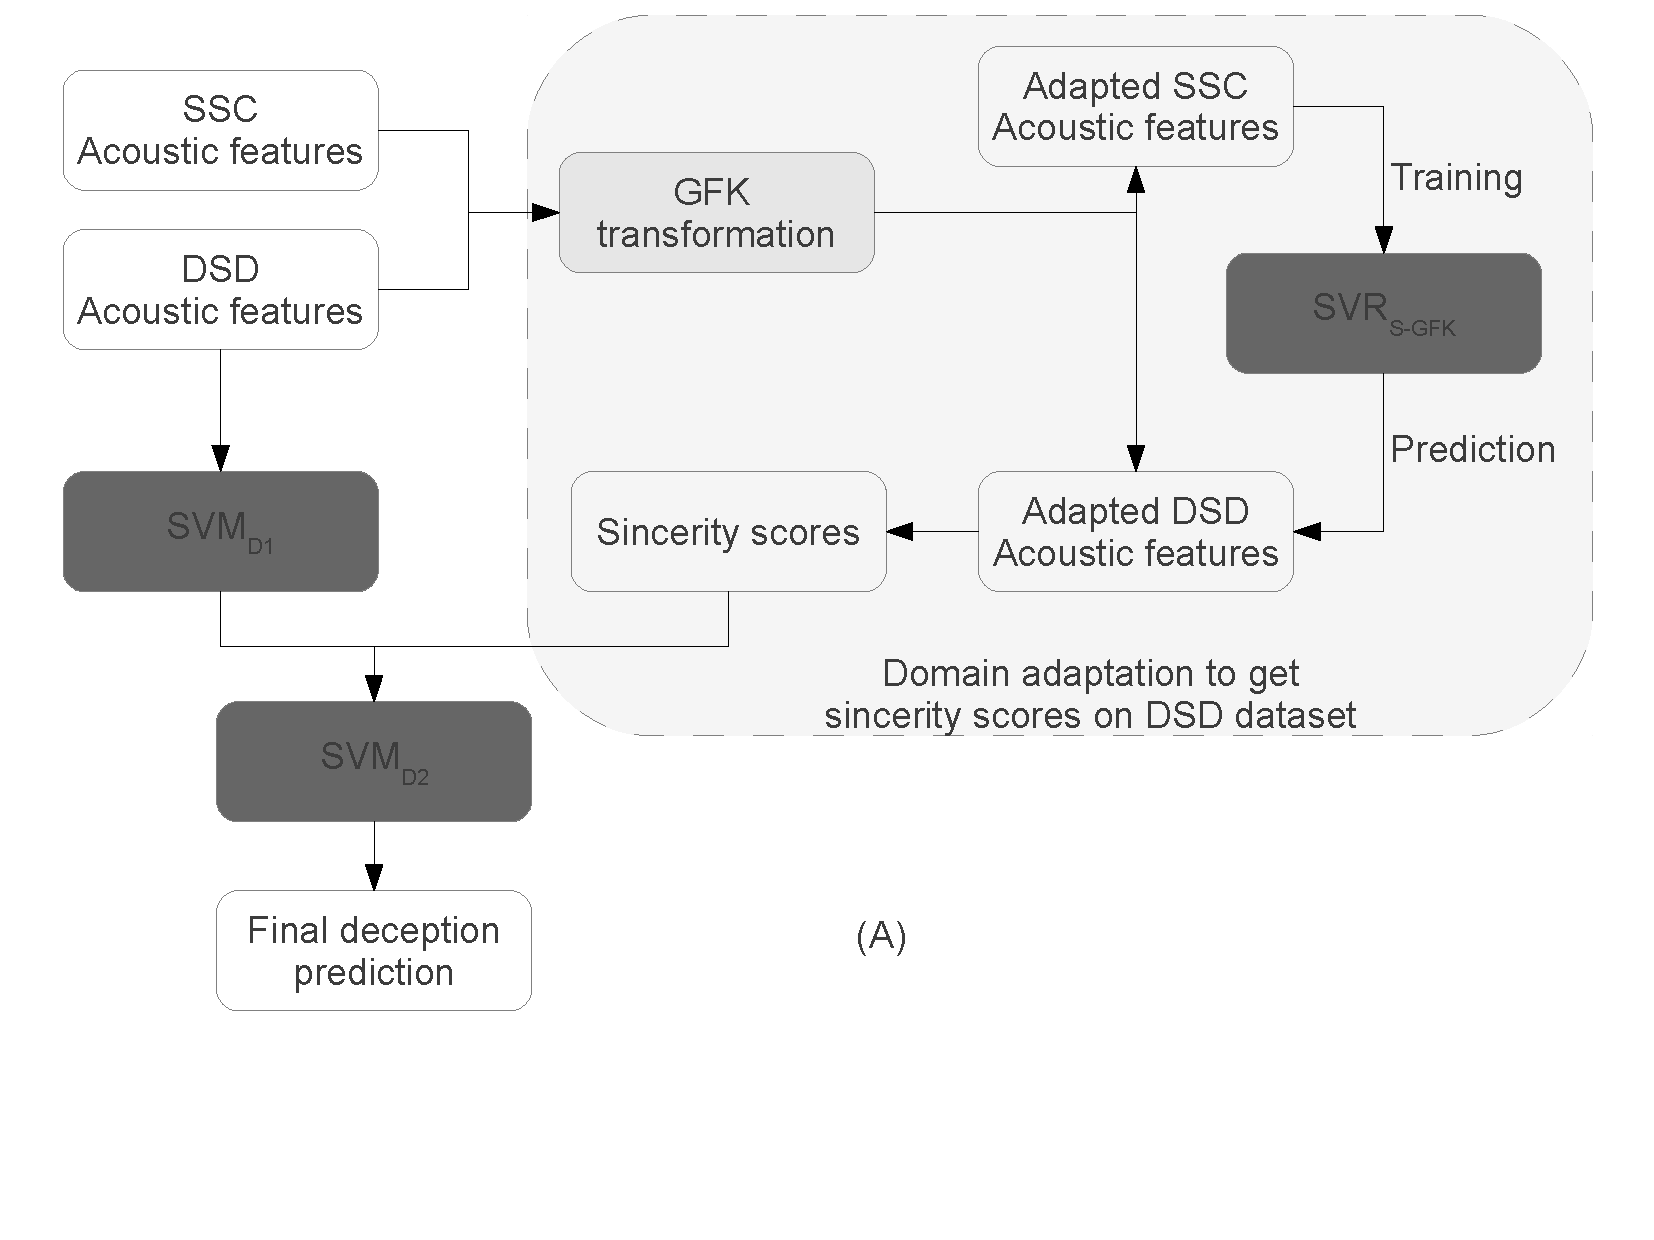
\includegraphics [trim=0cm 3.5cm 1cm 0cm,clip=true,scale=.3] {model_dec.pdf} 
%\end{subfigure}
%\begin{subfigure}{.5\textwidth}
%\centering
%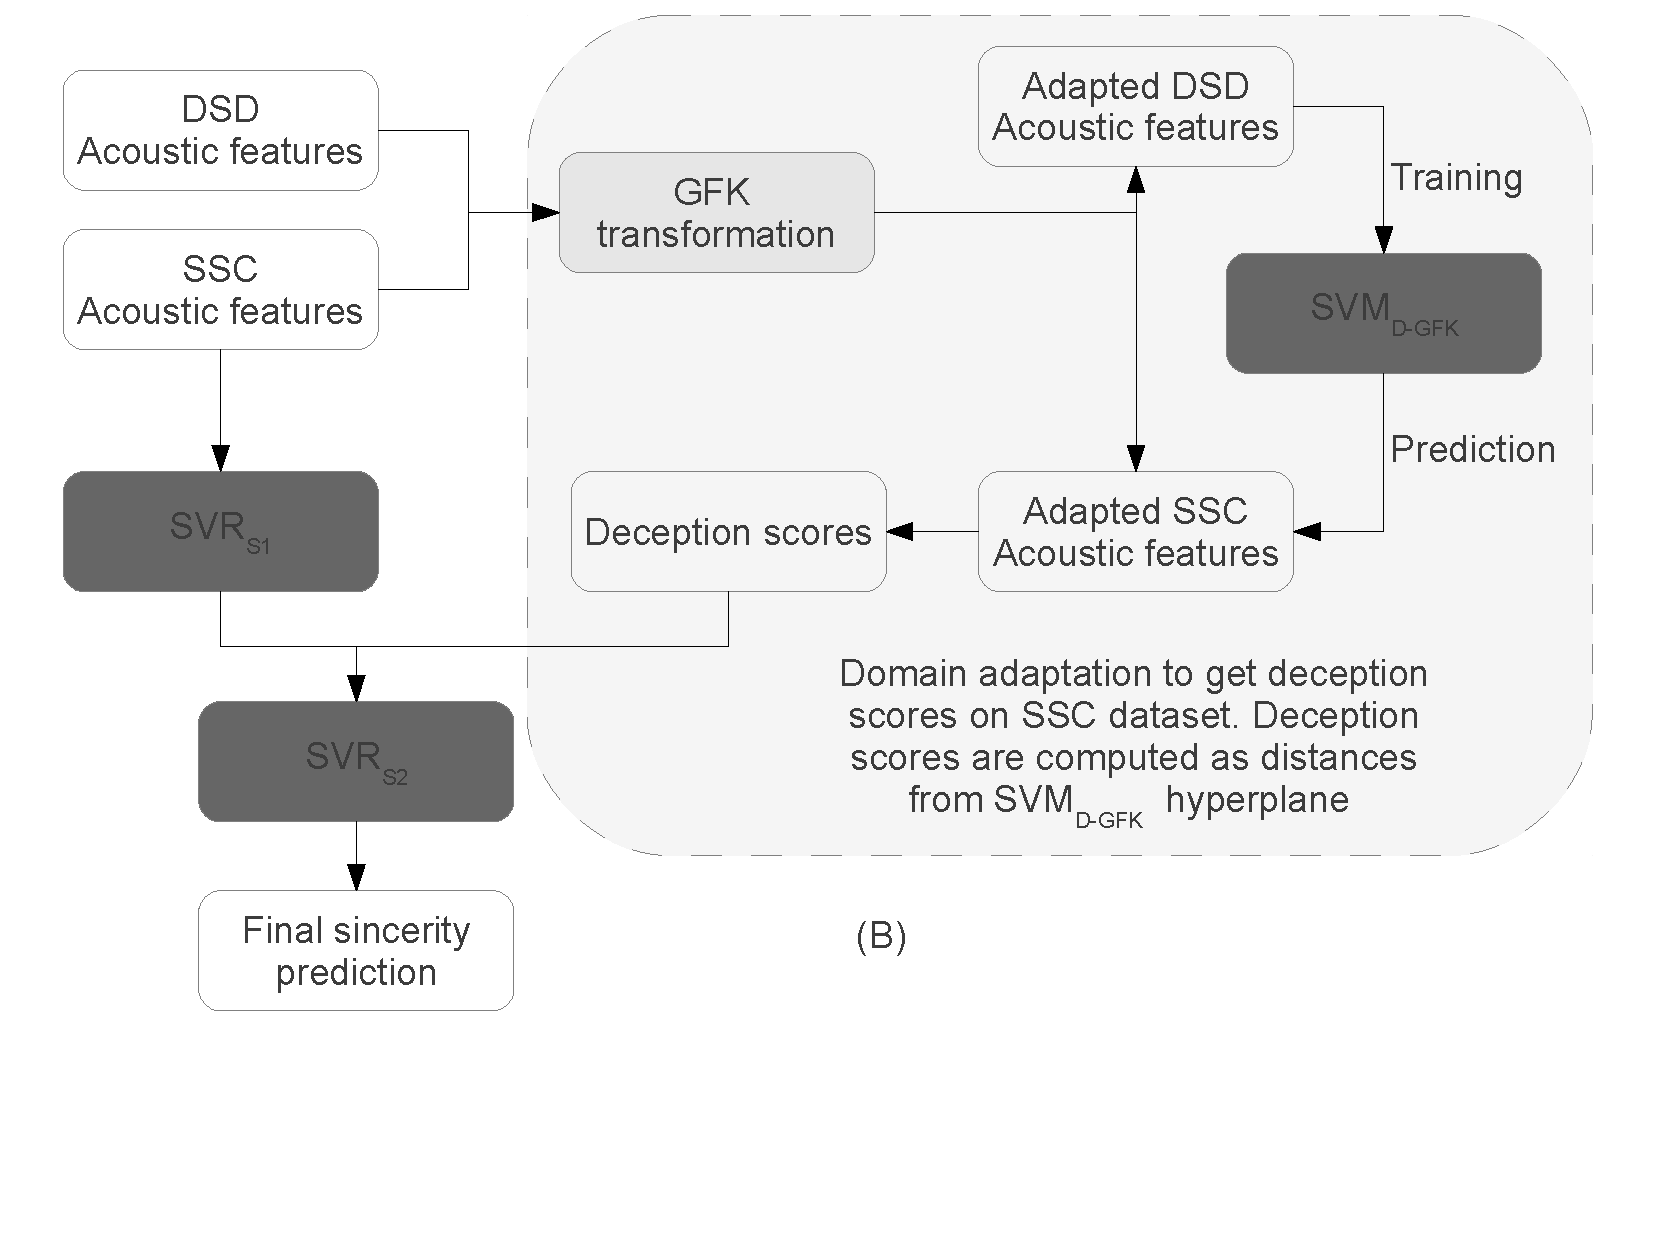
\includegraphics [trim=0cm 3.5cm 1cm 0cm,clip=true,scale=.3] {model_sinc.pdf} 
%\end{subfigure}
%\caption{Deception prediction using sincerity scores as features. Sincerity scores are obtained on adapted DSD dataset from SVR$_\text{S-GFK}$ which is trained on adapted SSC dataset.}
%\label{fig:dec_fig}
%\end{figure*}

\begin{figure*}[t]
\vspace{-8mm}
\begin{center}
\begin{tabular}
{@{\hspace{-0.0cm}}c@{\hspace{0.1cm}}c@{\hspace{0.0cm}}}
\raisebox{-.5\totalheight}{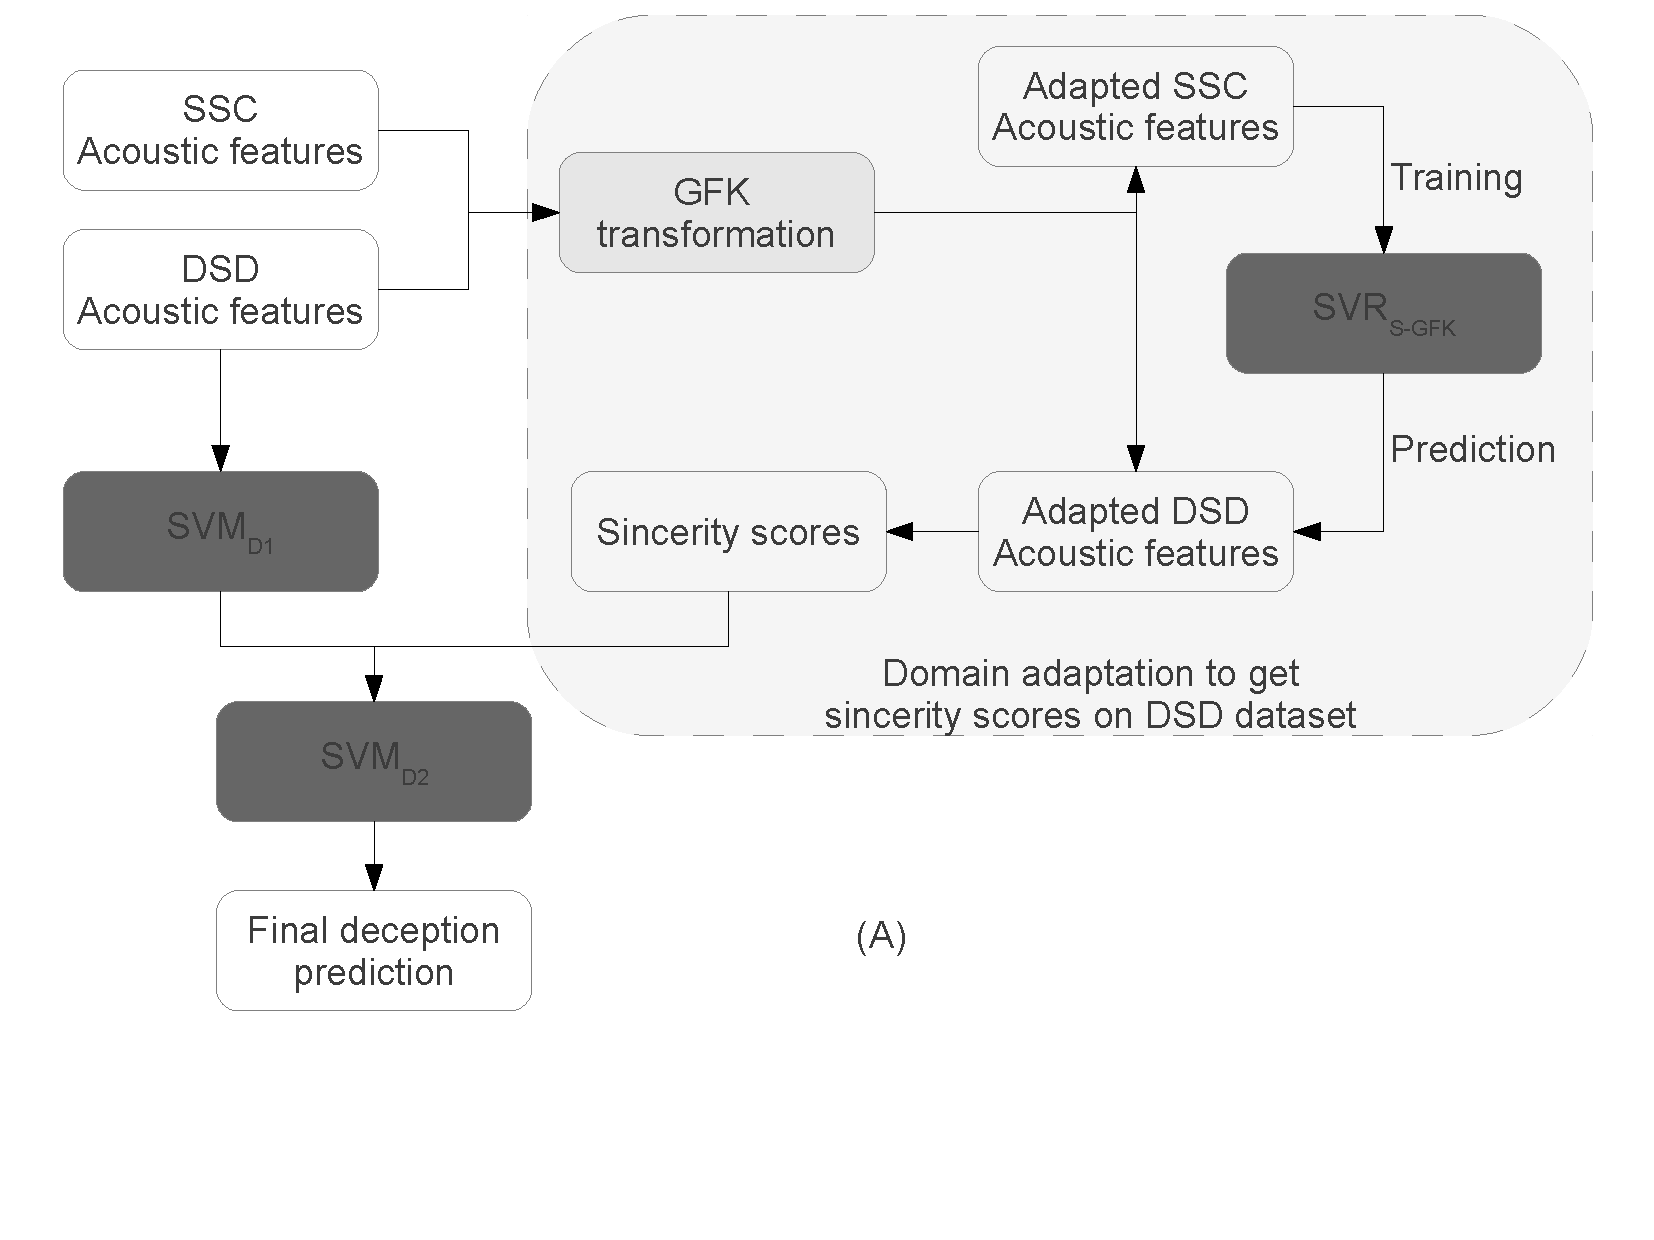
\includegraphics[trim=0cm 3cm 0cm 0cm,clip=true,scale=0.3]{model_dec.pdf}} &
\raisebox{-.495\totalheight}{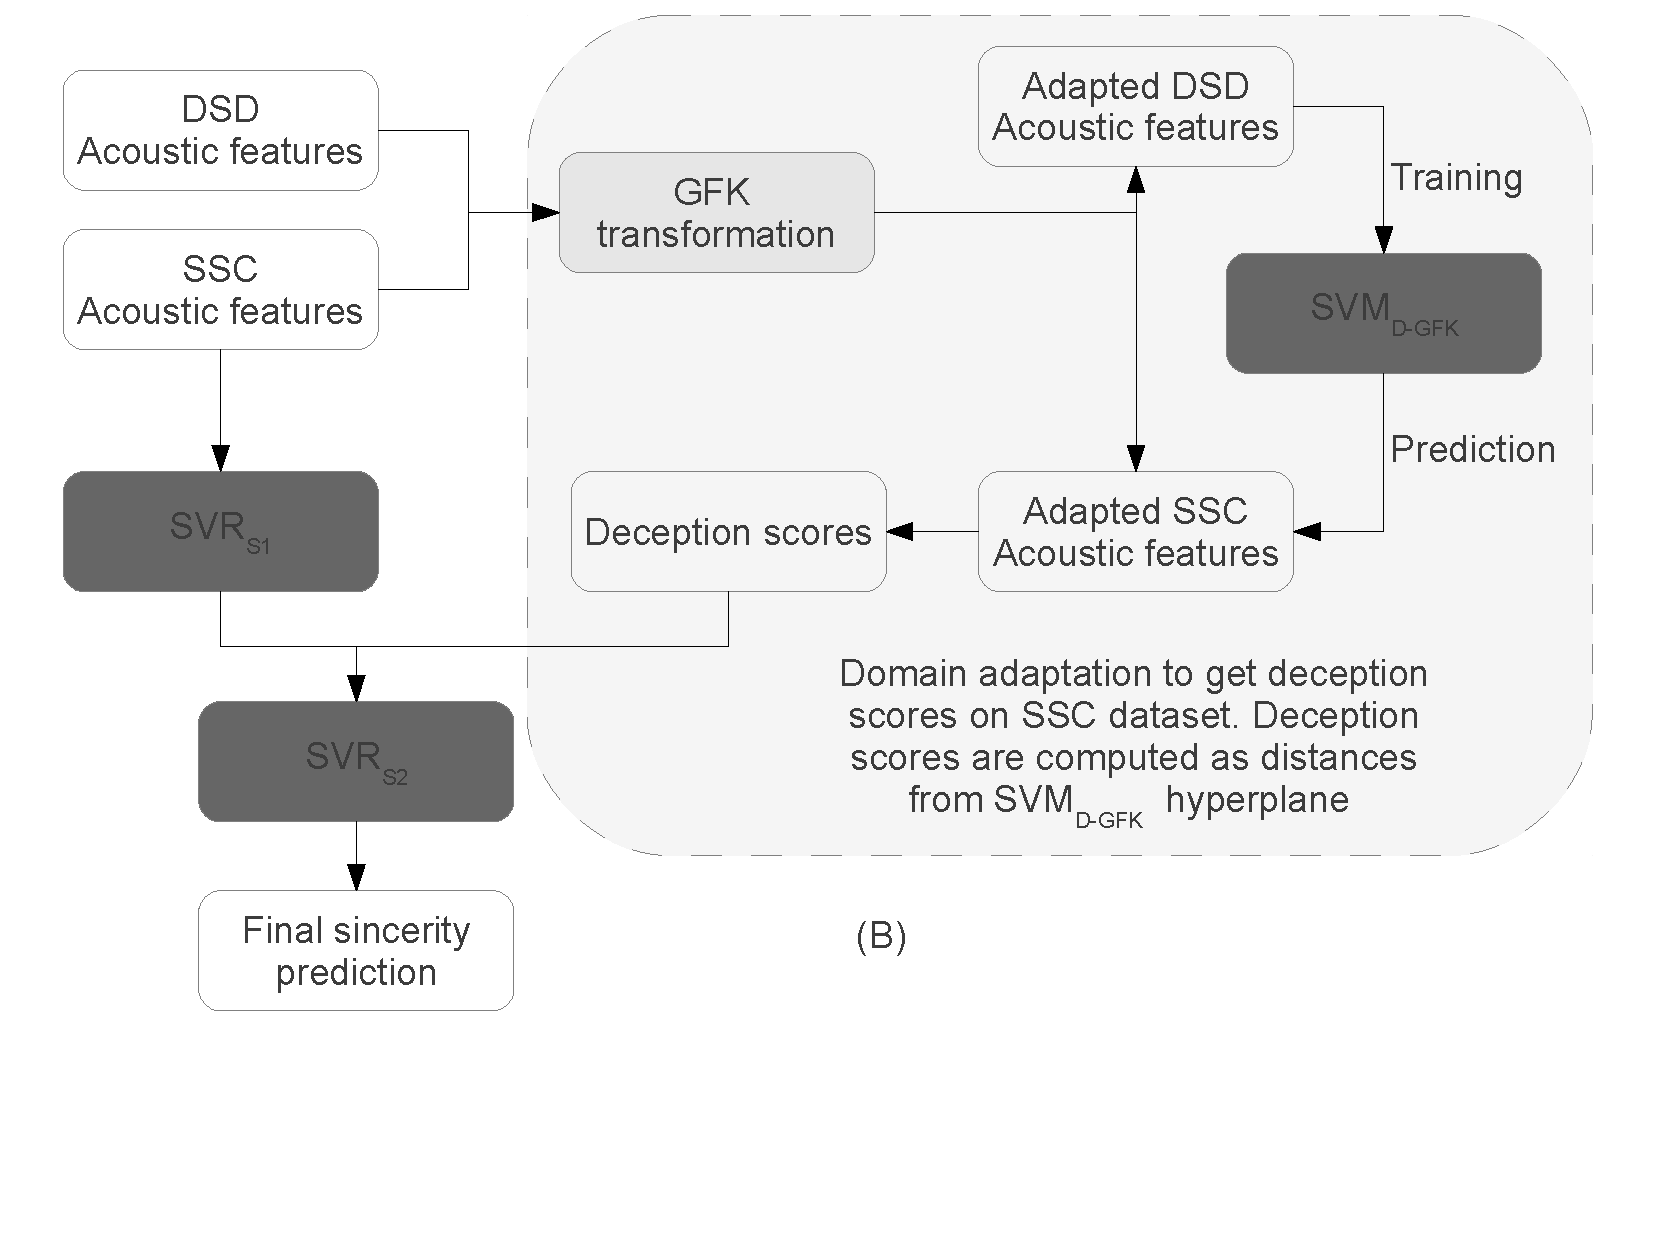
\includegraphics[trim=0cm 3cm 0cm 0cm,clip=true,scale=0.3]{model_sinc.pdf}}\\
\end{tabular}
%\renewcommand{\tabcolsep}{6pt}
\end{center}
\vspace{-9mm}
\caption{Stacked generalization framework for predicting: (a) Deception on DSD dataset (b) Sincerity on SSC dataset.}
\vspace{-6mm}
\label{fig:models}
\end{figure*}

%\noindent
\underline{\it Sincerity prediction}:
Akin to the deception prediction experiments, we use the predefined train, test and development set partitions for the SSC dataset.
In order to obtain deception predictions on the SSC dataset, we train an SVM model, SVM$_\text{D-GFK}$, on an adapted version of the DSD dataset.
The adaptation is again performed using the GFK transformation, with DSD dataset modified as source dataset to resemble SSC dataset as the target dataset.
Instead of using the binary deception labels from SVM$_\text{D-GFK}$ on SSC dataset, we again use distance of datapoints from SVM decision hyperplanes as a soft deception score estimate. 
We combine these deception scores with the original acoustic features again using a stacked generalization framework. 
A first layer SVR model (SVR$_\text{S1}$), trained on the SSC training partition, predicts the sincerity scores based on the original features (this model is same as the baseline sincerity prediction model). 
A second layer SVR model (SVR$_\text{S2}$) then combines the predictions from SVR$_\text{S1}$ with the deception scores from SVM$_\text{D-GFK}$ to provide the final sincerity scores.  
SVR$_\text{S2}$ is trained on the concatenated train and development sets to prevent overfitting to the training set.
Figure~\ref{fig:models}(B) summarizes the stacked generalization model for sincerity prediction. 
In the next section, we combined the adding datapoints and appending sincerity/deception outcomes as features. 

\vspace{-2mm}
\subsubsection{TL: adding datapoints + using sincerity/deception predictions as features}
\vspace{-2mm}
As the next step, we combine the previous two TL approaches of adding datapoints and sincerity/deception predictions as features.
We describe this approach below.
%\\

%\noindent
\underline{\it Deception prediction}: 
This experiment is similar to the deception prediction in the last section involving the incorporation of sincerity/deception scores as features during prediction.
The only difference is in the first stage of stacked generalization where we also append the SSC dataset to the DSD training partition to learn SVM$_\text{D1}$. 
SVM$_\text{D1}$ could be trained using either RANSAC or label transformation.
The second stage SVM, SVM$_\text{D2}$ is then trained on the DSD training and development partitions using the hyperplane distances predicted from SVM$_\text{D1}$ and the sincerity scores predicted by SVR$_\text{S-GFK}$. 
The final predictions on the DSD testing set are made by SVM$_\text{D2}$.
%\\

%\noindent
\underline{\it Sincerity prediction}:
We modify the first stage of stacked generalization as presented for sincerity prediction in Section~\ref{sec:gfkonly} by adding the DSD dataset to the SSC training partition in learning SVR$_\text{S1}$.
SVR$_\text{S1}$ is trained either using RANSAC or label transformation. 
In the second stage of stacked generalization, SVR$_\text{S2}$ is then trained on combined training and development sets with outcomes from SVR$_\text{S1}$ and SVM$_\text{D-GFK}$ as features.
We again use distances from SVM$_\text{D-GFK}$ as features as soft estimates of deception labels. 
SVR$_\text{S2}$ provides the final decisions on the SSC testing set.

In the next section, we present our results for the baseline and various TL models and present discussion.

%\subsubsection{Proposed method}
%The proposed method also exploited both data information and label information. However, unlike the aforementioned two methods, it implemented fusion of labels instead of combining the two datasets, and utilized a kernel-based domain adaptation method to reduce influence of differences in the recording conditions. In general, each data point was assigned 2 labels, one predicted by a D classifier and the other by a S regressor. The two labels were then combined to give a final decision.\par
%To predict labels for samples in one dataset using the training material of the same dataset, i.e. to predict labels for the D dataset using a D classifier and to predict labels for the S dataset using a S regressor, we made use of the classifiers and regressors from section 4.1, 4.2.1 and 4.2.2. The only difference was that the classifiers and regressors here were trained on their corresponding train sets only, while they were originally trained on the concatenated train and development sets. This was to ensure that the predictors here didn't see any data points in the development set, so it could still be reasonable to tune parameters for the fusion on the development set. The optimal box constraint and the optimal cost parameter were also obtained on the development set. In addition, in hope to obtain better performance, we tried to combine the aforementioned three methods by selecting the classifier/regressor that performed the best on the development set. After the prediction, for fusion of labels for the D dataset, distances from the decision hyperplane were used, because they contained more information than the binary labels. For S samples, we used the predicted sincerity ratings for fusion.\par
%To predict labels for samples in one dataset with a predictor trained on the other dataset, differences in data characteristics between the two datasets must be dealt with. This is because samples from one corpus can be very different from samples with the same degree of sincerity from the other corpus, which highly likely leads to wrong predictions. To ameliorate the differences, we performed unsupervised domain adaptation using Geodesic Flow Kernel (GFK). The GFK domain adaptation method aims to make datasets from different domains become more similar. It constructs a continuous transition from the source domain to the target domain, and along the way finds the best point for subspace projection, so that after the projection, low-dimensional domain-invariant representations of the two datasets can be derived. For more information, please refer to [x].\par
%After the transformation, a classifier was trained on the transformed D dataset to predict labels for the transformed S dataset, and we used the distance from the decision hyperplane for fusion as it contained more information. Similarly, a regressor was trained on the transformed S dataset to predict sincerity ratings for the transformed D dataset, and the labels were later used for fusion.\par
%For ease of notation, labels for one dataset that were predicted by a model trained on the same dataset are denoted as $Lbl_{orig}$, and those that were predicted by a model trained on the other dataset are denoted as $Lbl_{other}$.\par
%After the 2 labels were derived, they were both transformed into probability values by f(x) = exp(x)/[1+exp(x)]. Then different fusion strategies were adopted for D classification and S regression. For D classification, a combined decision was given by P = $\lambda$$P_{orig}$+(1-$\lambda$)$P_{other}$, where $P_{orig}$ and $P_{other}$ denoted the 2 probability values given by f(x). The parameter $\lambda$ was tuned on the development set, and the final binary labels were obtained by comparing P to 0.5. For S regression, a final decision was given by SVM regression on the 2 probability values. The cost parameter was tuned on the development set, and the test set performance was obtained using a model trained on the concatenated train and development sets.\par
%As a comparison, We tested another set of results using $Lbl_{other}$ alone (without transforming the labels into probability values). we also tried removing the GFK domain adaptation when testing with $Lbl_{other}$. Note that using $Lbl_{orig}$ alone would be the same as the methods in section 4.1, 4.2.1 and 4.2.2, therefore results in these three sections would automatically be a good comparison to the results of our proposed method.



\vspace{-3mm}
\section{Results and Discussion}
\vspace{-3mm}
Table~\ref{tab:results} shows the results for the various deception and sincerity prediction experiments. 
For the last TL experiment involving both adding of datapoints and using sincerity/deception predictions as features, we perform an additional experiment where the method for training SVM$_\text{D1}$ and SVR$_\text{S1}$ (RANSAC/ Label transformation/ not adding other dataset) for each cross-validation fold is chosen based on their performances on the development set. 
We perform this experiment to get a fair assessment of the TL on the test set, instead of advocating for a TL approach solely based on the results observed on the test set (a scenario not possible in the real world).

%\vspace{-3mm}
%\subsection
{\bf Discussion:}
%\vspace{-2mm}
From the results in Table~\ref{tab:results}, we observe that the additional information provided in the other datasets has minimal positive impact, with only RANSAC shows improvements in case of deception prediction.
This may stem from the fact that the labels are synthetically generated, as well as that the distribution of the datasamples in DSD and SSC datasets are not similar due to difference in recording conditions and data collection protocols. 
Therefore, adding the other dataset with synthetic labels only serves as a source of noise.
On the other hand, adding sincerity/deception scores after domain adaptation improves over the baseline. 
The UAR improvement is significant in case of deception prediction using McNemar test (p$<$5\%) modified for UAR, accounting for data imbalance \cite{bone2015applying}.
The improvement in Spearman's correlation for SSC dataset is not significant using Fisher r-to-z transformation, although the Pearson's correlation does show a marginally significant improvement (Fisher r-to-z transformation, p$<$10\%). 
Finally, adding datapoints from other dataset along with using sincerity/deception scores as features again gives mixed results with improvements only for label transformation. 
We are encouraged to see that the final assessment on the test set by tuning the method shows improvement for both the tasks over the baseline.
Although the performance for deception detection is worse off than only using model prediction as features, tuning provides the best overall performance for the sincerity task. 
% In summary, our experiments encourage us to further investigate TL methods is such 

In particular, we observe that using sincerity/deception scores as features during prediction delivers promising results.
On computing the absolute Spearman's correlation coefficient values between the predictions from SVR$_\text{S-GFK}$ and the true deception labels, we obtain a value of 19.1\%.
Similarly the absolute correlation coefficient between the deception scores obtained from SVM$_\text{D-GFK}$ and the true sincerity scores is 20.2\%.
Although these correlation coefficients are modest, they show meaningful correlation trend with deceptive labels having a low sincerity score and vice versa (in both the transformation experiments).  
Adding datapoints from the other dataset does not always improve the performance, therefore indicating that the synthetic label generation needs improvements. 
One future work in this regard is addressing the difference between the datasets while generating synthetic labels. 

 
%%Generally speaking, the performance improved after the fusion of labels, no matter which classifier/regressor was used to derive $Lbl_{orig}$. It did matter, however, whether the GFK domain adaptation was used to obtain $Lbl_{other}$, as shown in the table that without the domain adaptation, $Lbl_{other}$ would very much resemble random guessing. When using $Lbl_{orig}$ only, i.e. using the methods in 4.2.1 and 4.2.2 and their combination with the baseline method, the performance didn't show improvement in most cases as compared to the baselines.\par
%%In deception recognition, \par

\begin{table}
\caption{Results for predicting binary deception labels and sincerity scores on the DSD and SSC datasets, respectively. 
We report Unweighted Average Recall (UAR) for DSD dataset and Spearman's/Pearson's correlation coefficients ($\rho_s$/$\rho_p$) for the SSC dataset.
Best performances are marked in bold.}
\vspace{-4mm}
\centering
\begin{tabular}{@{}l|l|l@{}} \hline
            & Deception  & Sincerity  \\ 
            & (UAR in \%) & ($\rho_s, \rho_p$ in \%) \\ \hline
Baseline & 69.64 & 46.51, 41.58 \\ \hline
\multicolumn{3}{c} {TL: adding datapoints from other dataset} \\ \hline 
RANSAC & 70.26 & 46.45, 33.66 \\
Label Transformation & 67.17 & 43.44, 29.36 \\ \hline
\multicolumn{3}{c} {TL: Sinc./Dep. model prediction as features} \\ \hline 
 & \bf 72.02 & 48.53, 47.84 \\ \hline 
\multicolumn{3}{c} {TL: adding datapoints + Sinc./Dep. scores as features} \\ \hline 
+ RANSAC & 72.02 & 48.50, 48.04 \\ 
+ Label transformation & 69.90 & 49.37, 48.18\\
+ Tuned & 70.59 & \bf 49.37, 48.52 \\\hline 
\end{tabular}
\vspace{-6mm}
\label{tab:results}
\end{table}

%\centerline{Table1. UAR in deception recognition}
%\begin{threeparttable}
%\begin{tabular}{|l|l|l|l|}
%\hline
%& Using $Lbl_{orig}$ & Using $Lbl_{other}$ & Using fusion of\\
%& only & only & the 2 labels\\
%\hline
%Baselines & 0.6964 & \multirow{4}{*}{ } & 0.7202 \\
%\cline{1-2}
%\cline{4-4}
%RANSAC & (a) 0.6964\tnote{1} & 0.6081 & (a) 0.7202 \\
%& (b) 0.6964 & & (b) 0.7193 \\
%& (c) 0.7026 & & (c) 0.7096 \\
%\cline{1-2}
%\cline{4-4}
%Transform & 0.6717 & *w/o GFK: & 0.6990 \\
%labels & & 0.5275 & \\
%\cline{1-2}
%\cline{4-4}
%Combined\tnote{2} & (a)  & & (a) 0.7005 \\
%& (b)  & & (b) 0.7005\\
%& (c) 0.6933 & & (c) 0.7059\\
%\hline
%\end{tabular}
%\begin{tablenotes}
%\item[1] Listed in the table are results of the three strategies we applied. The strategies are: (a) add 5 percent of unlabeled data in each iteration; (b) add 5 percent of unlabeled data in each iteration; (c) add all of the unlabeled data in one iteration. Please refer to section 4.2.1 for more details.
%\item[2] In the combined method, as stated in 4.2.3, the three methods above were integrated by selecting the classifier that performed the best on the development set in each fold. The said classifier was then used in the fusion. The identifier (a), (b), (c) indicates which RANSAC strategy was used.
%\end{tablenotes}
%\end{threeparttable}
%
%\medskip
%
%\centerline{Table2. Spearman's correlation in sincerity evaluation}
%\begin{threeparttable}
%\begin{tabular}{|l|l|l|l|}
%\hline
%& Using $Lbl_{orig}$ & Using $Lbl_{other}$ & Using fusion of\\
%& only & only & the 2 labels\\
%\hline
%Baselines & 0.4651 (0.4158\tnote{1}) & \multirow{4}{*}{ } & 0.4853 (0.4784) \\
%\cline{1-2}
%\cline{4-4}
%RANSAC & 0.4645\tnote{2} (0.3366) & 0.1867 (0.1755) & 0.4850 (0.4804) \\
%\cline{1-2}
%\cline{4-4}
%Transform & 0.4344 (0.2936) & *w/o GFK: & 0.4937 (0.4818) \\
%labels & & 0.0084 (0.0101) & \\
%\cline{1-2}
%\cline{4-4}
%Combined\tnote{3} & 0.4590 (0.3108) & & 0.4896 (0.4738) \\
%\hline
%\end{tabular}
%\begin{tablenotes}
%\item[1] To conduct significance tests, Pearson's correlation was also computed and is shown in parentheses in the table.
%\item[2] Between the two strategies we applied, only the best result is shown in the table. The strategy that generated the best result was then used in the fusion, while the other was not. Both two results are as follows: (a) add one cluster of the unlabeled data in each iteration: 0.4645; (b) add all of the unlabeled data in one iteration: 0.4351.
%\item[3] In the combined method, as stated in 4.2.3, the three methods above were integrated by selecting the regressor that performed the best on the development set in each fold. The said regressor was then used in the fusion.
%\end{tablenotes}
%\end{threeparttable}
%

\vspace{-3mm}
\section{Conclusion}
\vspace{-3mm}

Transfer Learning has shown promise in several domains including human behavior modeling, where it can be expensive and time prohibitive to obtain large amounts of appropriately labeled data.
In this work, we apply TL methods to the problems of sincerity and deception prediction using behavioral data from two distinct datasets; the DSD and SSC datasests. 
We test two methods: (i) adding datapoints from the other dataset and, (ii) appending system predictions from the other tasks as features. 
%using sincerity predictions learnt on SSC dataset as features for deception prediction (likewise for sincerity prediction using deception models learnt on DSD dataset). 
We also test a combination of the two methods and present our analysis.
We obtain superior performances to models trained only on in-domain data, indicating the promise of TL methods in such problems. 

In the future, we aim to explore other methodologies within the domain of TL to the problem of sincerity and deception prediction (e.g. other domain adaptation methods \cite{jiang2008literature}).
One could also test the applied methods to other human behavior modeling domains such as engagement \cite{gupta2016analysis} and interestingness \cite{freitas1999rule}.
Finally, we are also working on formulating a theoretical understanding of the transfer of knowledge between correlated concepts with differences in data recording conditions. 
\end{spacing}

\footnotesize
{
%\begin{spacing}{0.87}
%\vfill\pagebreak
% BiBTeX files (here: strings, refs, manuals). The IEEEbib.bst bibliography
% style file from IEEE produces unsorted bibliography list.
% -------------------------------------------------------------------------
\bibliographystyle{IEEEbib2}
\bibliography{strings,refs}
%\end{spacing}
}
\end{document}
